% !Mode:: "TeX:UTF-8"
% !TEX program  = xelatex
\title{Assignment 1}
\maketitle

\section{Question 1}\label{S:1}
\begin{statebox}{}{question-1}
    What would you do to make money if all you had was \emph{100 RMB} and \emph{8 hours}.
\end{statebox}
If I have ¥100 and 8 hours, I will not invest in stocks or options until I learn the financial basics, therefore I have to take a different approach to making money. Please see Question~\ref{S:3}.



\section{Question 2}\label{S:2}
\begin{statebox}{}{question-2}
    Find the top 10 best sellers in computational finance, home and abroad and share with others.
\end{statebox}
The top 10 best quantitative finance books I find in \href{https://www.wallstreetmojo.com/top-best-quantitative-finance-books/}{WallStreetMojo} is:\cite{Dheeraj2016finace-books}
\begin{enumerate}
    \item \emph{An Introduction to Quantitative Finance}
        \hfill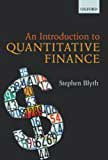
\includegraphics[height=.5in]{figures/2019-09-17-finance-books-1.jpg}
    \item \emph{Quantitative Trading with R}
        \hfill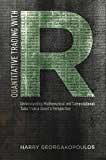
\includegraphics[height=.5in]{figures/2019-09-17-finance-books-2.jpg}
    \item \emph{Quantitative Momentum}
        \hfill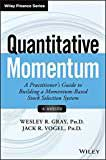
\includegraphics[height=.5in]{figures/2019-09-17-finance-books-3.jpg}
    \item \emph{Quantitative Finance For Dummies}
        \hfill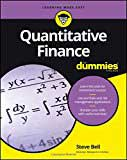
\includegraphics[height=.5in]{figures/2019-09-17-finance-books-4.jpg}
    \item \emph{Finance: A Quantitative Introduction}
        \hfill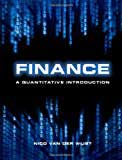
\includegraphics[height=.5in]{figures/2019-09-17-finance-books-5.jpg}
    \item \emph{Quantitative Methods for Business}
        \hfill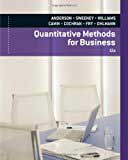
\includegraphics[height=.5in]{figures/2019-09-17-finance-books-6.jpg}
    \item \emph{Quantitative Methods for Finance}
        \hfill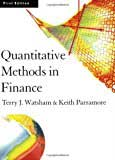
\includegraphics[height=.5in]{figures/2019-09-17-finance-books-7.jpg}
    \item \emph{Quantitative Risk Management}
        \hfill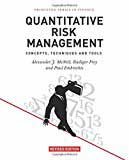
\includegraphics[height=.5in]{figures/2019-09-17-finance-books-8.jpg}
    \item \emph{Quantitative Finance}
        \hfill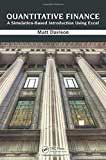
\includegraphics[height=.5in]{figures/2019-09-17-finance-books-9.jpg}
    \item \emph{Extreme Financial Risks and Asset Allocation}
        \hfill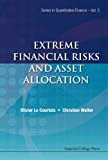
\includegraphics[height=.5in]{figures/2019-09-17-finance-books-10.jpg}
\end{enumerate}



\section{Question 3}\label{S:3}
\begin{statebox}{}{question-3}
    Try to create an account with 10k RMB and keep simulated trading for the rest of the semester.
\end{statebox}
The website I use to simulate trading is \href{https://www.ricequant.com/quant/}{RiceQuant}, which has some \texttt{Python} modules called \verbbox{rqalpha}, \verbbox{rqfactor}, etc. Since I am new to the computational finance, there is a lot of basics about finance I need to learn. Therefore when finishing learning the financial basics, I will create an account and keep simulated trading for the rest of the semester, now I have read the API documentation of the RiceQuant, but without the theoretical support, what I can do is limited, here comes the first getting-started strategy I have learned in the RiceQuant:
\begin{pylist}{RiceQuant}
def init(context):
    context.s1 = "000001.XSHE"
    logger.info("Interested at stock: " + str(context.s1))

def before_trading(context):
    pass

def handle_bar(context, bar_dict):
    order_shares(context.s1, 1000)
\end{pylist}\label{C:rice-quant-getting-started}

And the figure~\ref{F:ricequant-getting-started} shows the result of the first strategy.
\begin{figure}
    \centering
    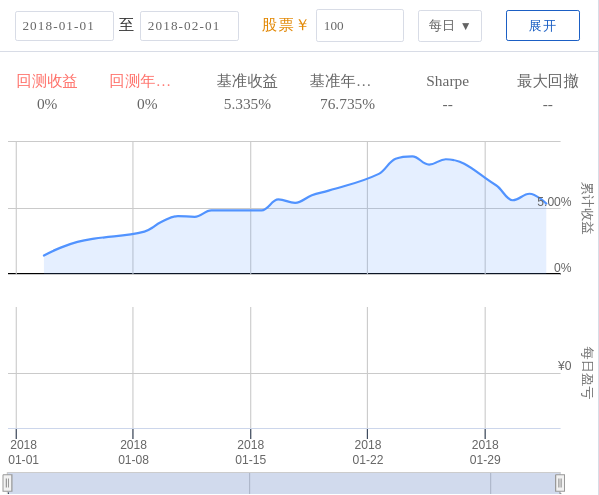
\includegraphics[width=\textwidth]{figures/2019-09-17-qicequant.jpg}
    \caption{Result in RiceQuant}\label{F:ricequant-getting-started}
\end{figure}



\bibliography{ref}
